\section{\secarithtriangle}
\label{sec_arith_triangle}

In \Cref{ch_counting}, we saw three counting techniques: steps (where we multiply), cases (where we add), and subsets (where we use binomial coefficients).  In \Cref{sec_model_sum_prod} and \Cref{sec_sum_conj}, we worked with sums and products.  In this section, we revisit the binomial coefficients, defined in \Cref{defn_binomial_coeff}, which are 
    $$ \binom{n}{k} = \text{ the number of ways to select a subset of } k \text{ elements from a set of } n \text{ elements}$$ 
for nonnegative integers $n$ and $k$.
We introduce the arithmetic triangle.\footnote{The arithmetic triangle was formerly known as Pascal's triangle, and the generic name honors that the arithmetic triangle was known in Asia, the middle East, and Europe countries centuries before Pascal lived.} We examine the recursion that generates the arithmetic triangle, which is useful for computation, and search for patterns among the binomial coefficients, including summations.  We also explain the origin of the name ``binomial coefficient'' and we derive an explicit formula for the binomial coefficients which is of theoretical use.

%%%%%%%%%%%%%%%%%%%%%%%%%%%%%%%%%%%%%%%%%%
\newcommand{\subarithtri}{The Arithmetic Triangle}
\subsection{\subarithtri}
\label{sub_arith_triangle}

How do we calculate the value of $\binom{n}{k}$?  Let's first look at an example using the definition.

\begin{exam}[Evaluating a binomial coefficient by listing subsets]
\label{exam_eval_7choose4}
    Evaluate $\binom{7}{4}$ without using computational technology.
        \begin{soln}
            By \Cref{defn_binomial_coeff}, we can count all 4-element subsets of a set with seven elements, say $\{1,2,3,4,5,6,7\}$. We list these subsets in \Cref{table_subset_list_7choose4}.  There are 35 subsets, so $\binom{7}{4}=35.$

                \begin{table}[hbtp]
                \centering
                \begin{tabular}{ccccc}
                    $\{1,2,3,4\}$ & 
                    $\{1,2,3,5\}$ &
                    $\{1,2,3,6\}$ &
                    $\{1,2,3,7\}$ &
                    $\{1,2,4,5\}$ \\
                    $\{1,2,4,6\}$ & 
                    $\{1,2,4,7\}$ &
                    $\{1,2,5,6\}$ &
                    $\{1,2,5,7\}$ &
                    $\{1,2,6,7\}$ \\
                    $\{1,3,4,5\}$ & 
                    $\{1,3,4,6\}$ &
                    $\{1,3,4,7\}$ &
                    $\{1,3,5,6\}$ &
                    $\{1,3,5,7\}$ \\
                    $\{1,3,6,7\}$ & 
                    $\{1,4,5,6\}$ &
                    $\{1,4,5,7\}$ &
                    $\{1,4,6,7\}$ &
                    $\{1,5,6,7\}$ \\
                    $\{2,3,4,5\}$ & 
                    $\{2,3,4,6\}$ &
                    $\{2,3,4,7\}$ &
                    $\{2,3,5,6\}$ &
                    $\{2,3,5,7\}$ \\
                    $\{2,3,6,7\}$ & 
                    $\{2,4,5,6\}$ &
                    $\{2,4,5,7\}$ &
                    $\{2,4,6,7\}$ &
                    $\{2,5,6,7\}$ \\
                    $\{3,4,5,6\}$ & 
                    $\{3,4,5,7\}$ &
                    $\{3,4,6,7\}$ &
                    $\{3,5,6,7\}$ &
                    $\{4,5,6,7\}$\\
                \end{tabular}
                \caption{The 4-element subsets of the set $\{1,2,3,4,5,6,7\}$.}
                \label{table_subset_list_7choose4}
            \end{table}
        \end{soln}
\end{exam}

There are some values of binomial coefficients that we can compute from the definition.

\begin{exam}[Border values of binomial coefficients]
\label{exam_border_values_binom_coeffs}
~
    \begin{apart}
        \item Explain why $\binom{n}{0}=1$ and $\binom{n}{n}=1$ using the definition of the binomial coefficients.
            \begin{soln}
                Given a set with $n$ elements, there is only one 0-element subsets, namely the empty set $\varnothing$.  Similarly, there is only one $n$-element subset, namely the set itself.
            \end{soln}
        \item Explain why $\binom{n}{1}=n$ using the definition of the binomial coefficients.
            \begin{soln}
                Given a set with $n$ elements, there are $n$ 1-element subsets, one for each element of the set.
            \end{soln}
    \end{apart}
\end{exam}

Listing the $k$-element subsets of a set with $n$ elements is tedious, even for small values of $n$ and $k$, and it is impractical for any larger values.  We would like a more efficient way to calculate the values of $\binom{n}{k}$ by hand for small values of $n$ and $k$.  For larger values, we seek a recursive definition to compute the values.  We begin with a way to list binomial coefficients in a triangular array.

\begin{defn}[The arithmetic triangle]
\label{defn_arith_triangle}
    The \vocab{arithmetic triangle} is an array of binomial coefficients, where each row has, in order, the values $\binom{n}{k}$, for $k=0,1,2, \ldots, n$. For example, the first row has a single value, $\binom{0}{0}=1$.  The second row has, in order, the values $\binom{1}{0}=1$ and $\binom{1}{1}=1$.  The third row has, in order, the values $\binom{2}{0}=1$, $\binom{2}{1}=2$, and $\binom{2}{2}=1$. \Cref{figure_arith_tri_expanded} shows the first eight rows of the expanded version of the arithmetic triangle that includes the binomial coefficients and their values. \Cref{figure_arith_tri_standard} shows the first eight rows of the standard version that lists only the values.

        \begin{figure}[hbtp]
            \centering
                $$\binom{0}{0}=1$$ 
                $$\binom{1}{0}=1 \hspace{.23in} \binom{1}{1}=1$$ 
                $$\binom{2}{0}=1 \hspace{.23in} \binom{2}{1}=2 \hspace{.23in} \binom{2}{2}=1$$ 
                $$\binom{3}{0}=1 \hspace{.23in} \binom{3}{1}=3 \hspace{.23in} \binom{3}{2}=3\hspace{.23in} \binom{3}{3}=1$$ 
                $$\binom{4}{0}=1 \hspace{.23in} \binom{4}{1}=4 \hspace{.23in} \binom{4}{2}=6 \hspace{.23in} \binom{4}{3}=4\hspace{.23in} \binom{4}{4}=1$$ 
                $$\binom{5}{0}=1 \hspace{.23in} \binom{5}{1}=5 \hspace{.23in} \binom{5}{2}=10 \hspace{.23in} \binom{5}{3}=10\hspace{.23in} \binom{5}{4}=5\hspace{.23in} \binom{5}{5}=1$$ 
                $$\binom{6}{0}=1 \hspace{.23in} \binom{6}{1}=6\hspace{.23in} \binom{6}{2}=15 \hspace{.23in} \binom{6}{3}=20\hspace{.23in} \binom{6}{4}=15\hspace{.23in} \binom{6}{5}=6\hspace{.23in} \binom{6}{6}=1$$ 
                $$\binom{7}{0}=1 \hspace{.23in} \binom{7}{1}=7\hspace{.23in} \binom{7}{2}=21 \hspace{.23in} \binom{7}{3}=35\hspace{.23in} \binom{7}{4}=35\hspace{.23in} \binom{7}{5}=21\hspace{.23in} \binom{7}{6}=7\hspace{.23in} \binom{7}{7}=1$$
            \caption{The first eight rows of the  arithmetic triangle in expanded format.}
            \label{figure_arith_tri_expanded}
        \end{figure}

        \begin{figure}
            \centering
                $$1$$
                $$1 \hspace{.23in} 1$$
                $$1 \hspace{.23in} 2 \hspace{.23in} 1$$
                $$1 \hspace{.23in} 3 \hspace{.23in} 3\hspace{.23in} 1$$
                $$1 \hspace{.23in} 4 \hspace{.23in} 6 \hspace{.23in} 4\hspace{.23in}1$$
                $$1 \hspace{.23in} 5 \hspace{.23in} 10 \hspace{.23in} 10\hspace{.23in} 5\hspace{.23in} 1$$
                $$1 \hspace{.23in} 6\hspace{.23in} 15 \hspace{.23in} 20\hspace{.23in}15\hspace{.23in} 6\hspace{.23in} 1$$
                $$1 \hspace{.23in} 7\hspace{.23in} 21 \hspace{.23in} 35\hspace{.23in} 35\hspace{.23in}21\hspace{.23in} 7\hspace{.23in} 1$$
            \caption{The first eight rows of the  arithmetic triangle in standard format.}
            \label{figure_arith_tri_standard}
        \end{figure}
\end{defn} 

We can use the arithmetic triangle to evaluate binomial coefficients.

\begin{exam}[Using the arithmetic triangle to evaluate binomial coefficients]
\label{exam_using_arith_tri_eval}
    Use the arithmetic triangle drawn in \Cref{figure_arith_tri_standard} to evaluate each binomial coefficient.  If you are not sure where to look in the triangle, refer to \Cref{figure_arith_tri_expanded}.
        \begin{apart}
            \item Evaluate $\displaystyle \binom{4}{2}$.
                \begin{soln}
                    The row that starts with 1, 4 lists $$\binom{4}{0}=1, \binom{4}{1}=4, \binom{4}{2}=6, \ldots.$$  This answer agrees with our list of the 2-element subsets of $\{1,2,3,4\}$ from \Cref{exam_four_choose_k}.
                \end{soln}
            \item Evaluate $\displaystyle \binom{6}{4}$.
                \begin{soln}
                    The row that starts with 1, 6 lists $\displaystyle \binom{6}{k}$ for $k=0, 1, 2, 3, 4, \ldots$. Because the list begins at $k=0$,  the fifth number in that row gives $$\displaystyle \binom{6}{4}=15.$$
                \end{soln}
        \end{apart}
\end{exam}

Try working with the arithmetic triangle.

\begin{act}[The arithmetic triangle]
\label{act_arith_tri}
~
    \begin{actpart}
        \item Copy the first eight rows of the arithmetic triangle. 
        \item Use the arithmetic triangle to evaluate each of the following binomial coefficients and circle the corresponding entries in the triangle.
        $$\binom{5}{4}, \binom{7}{5}, \binom{3}{0}, \binom{6}{1}, \binom{2}{2}.$$
        
        \item \label{part_arith_tri_from6to7} There is a way to calculate the row that starts with 1, 7 from the row above it.  Can you see how?  (Do not spoil the surprise for others if you already know the answer.) Hint: Each entry of the row is calculated using two nearby entries from the previous row.  
        
        \item \label{part_arith_tri_from7to8} Use the pattern from (\ref{part_arith_tri_from6to7}) to write the next row that starts with 1, 8.
        
        \item \label{part_eval_8choosek} Use your new row to evaluate each of the following binomial coefficients:
        $$ \binom{8}{2}, \binom{8}{4}, \binom{8}{5}.$$
        
        \item Write a formula for how to calculate the row that stars $1, n$ from the row above it.  Your formula should be in the form $\displaystyle \binom{n}{k} = .$  Hint: The entries from the row above will involve $n-1$ and $k$s.
    \end{actpart}
\end{act}

Make sure to complete \Cref{act_arith_tri} before reading on because we are going to share the key observation.

\begin{rem}[Generating the arithmetic triangle]
\label{rem_generating_arith_triangle}
    We can generate the arithmetic triangle as follows.
        \begin{apart}
            \item The first row is 1.  
            \item The entry in each subsequent row is the sum of the two entries above it in the previous row, with the understanding that a missing entry equals zero.  
        \end{apart}
\end{rem}

We state this recursion formally.

\begin{thm}[Recursive definition of the binomial coefficients]
\label{thm_pascals_recursion}
    The binomial coefficients can be defined recursively by $\binom{n}{0}=\binom{n}{n}=1$ and 
                $$\binom{n}{k}=\binom{n-1}{k-1} + \binom{n-1}{k}$$
    for any nonnegative integer $n$ and integer $k=1, \ldots, n-1$.
\end{thm}

Let's see this formula in action.

\begin{exam}[Adding another row to the arithmetic triangle]
\label{exam_arith_tri_row9}
    Use \Cref{thm_pascals_recursion} to write the row of the arithmetic triangle that begins with 1, 8.  
        \begin{soln}
            We begin with a copy of the row that begins with 1, 7 from \Cref{figure_arith_tri_standard}. We add neighboring entries to calculate the entries of the next row: $$ 0+1=1 \quad 1+7=8\quad 7 +21 = 28\quad 21+35 = 56\quad 35+35=70$$
            $$35+21 = 56\quad 21+7 = 28\quad 7+1 = 8\quad 1 + 0 = 1$$
            The result is shown in \Cref{fig_arith_triangle_recursion}.

                \begin{figure}[hbtp]
                    \centering
                    \scalebox{0.85}{%Used in \Cref{sec_arith_triangle}.

% Thank you Gemini!
% My prompt was: I'm writing a discrete math textbook.  We're learning about the arithmetic triangle (Pascal's triangle).  I want to illustrate how the recursion gets us from the row starting 1, 7 to the row starting 1,8.  The recursion is that you add the two numbers from the previous row. (Or you can look up Pascal's identity).  I have a graphic, which I'll paste at the end of this note.  I would like to replace it with a Tikz image that shows what I have , but adds line segments of slope 1 and -1 between entries of the top row and the bottom row as follows.  Negative slope lines from 1 to 8, from 7 to 28, from 21 to 56, etc.  Positive slope lines from 8 to 7 from 2 to 21, from 56 to 35, etc.  They can be blue and maybe the second row would also be blue??  Here's the existing rows: 

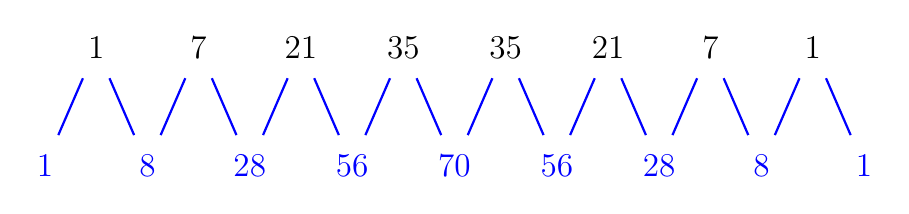
\begin{tikzpicture}[
    x=1.3cm, % Adjust horizontal spacing here. 1.3cm is approx 0.5in center-to-center
    y=1.5cm, % Adjust vertical spacing here
    every node/.style={font=\large, anchor=base},
    top row/.style={black},
    bottom row/.style={blue}
    ]

% --- Define data ---
\def\rowSeven{1, 7, 21, 35, 35, 21, 7, 1}
\def\rowEight{1, 8, 28, 56, 70, 56, 28, 8, 1}

% --- Place Row 7 (Top Row) ---
% These are offset horizontally by 0.5 units to sit between the row below
\foreach \val [count=\i from 0] in \rowSeven {
    \node[top row] (T-\i) at (\i + 0.5, 1) {$\val$};
}

% --- Place Row 8 (Bottom Row) ---
\foreach \val [count=\i from 0] in \rowEight {
    \node[bottom row] (B-\i) at (\i, 0) {$\val$};
}

% --- Draw Connections ---
\begin{scope}[blue, thick, shorten <=4pt, shorten >=4pt]
    % We iterate through the top row items (T-0 to T-7).
    % Each T-i connects to the node directly below-left (B-i)
    % and directly below-right (B-{i+1}).
    \foreach \i in {0,...,7} {
        % Define the index for the bottom right connection
        \pgfmathtruncatemacro{\nextB}{\i+1}

        % Line of positive slope (visually bottom-left to top-right)
        % Connects B-\i up to T-\i
        \draw (B-\i) -- (T-\i);

        % Line of negative slope (visually top-left to bottom-right)
        % Connects T-\i down to B-\nextB
        \draw (T-\i) -- (B-\nextB);
    }
\end{scope}

\end{tikzpicture}}
                    \caption{Generating another row of the arithmetic triange.}
                    \label{fig_arith_triangle_recursion}
                \end{figure}
        \end{soln}
\end{exam}

%%%%%%%%%%%%%%%%%%%%%%%%%%%%%%%%%%%%%%%%%%
\newcommand{\subpascalpatterns}{Patterns in the Arithmetic Triangle}
\subsection{\subpascalpatterns}
\label{sub_pascal_patterns}

There are many patterns that involve binomial coefficients.  

\begin{act}[Looking for patterns in the arithmetic triangle]
\label{act_pascals_patterns}
~
    \begin{exerpart}
        \item \label{part_arith_tri_sym_conj} Do you notice a symmetry in the arithmetic triangle?  State your observation as a conjecture of the form $\binom{n}{k}=\binom{n}{\quad}.$
        \item \label{part_find_row_sum_arith_tri} Calculate the sum of the entries in each of row of the arithmetic triangle. What did you notice?  State your observation as a conjecture, using summation notation for the sum.
        \item \label{part_alt_row_sum_arith_tri} Conjecture an explicit formula for the sum $$\sum_{k=0}^n(-1)^k\binom{n}{k}$$
        for $n \ge 0$.  Hint:  Calculate the sum when $n=3$ and $n=4$ first.
        \end{exerpart}
\end{act}

Let's look at the first two patterns from \Cref{act_pascals_patterns}.  We begin with the left-right symmetry.

\begin{thm}[Symmetry in the arithmetic triangle.]
\label{thm_sym_arith_triangle}
    For nonnegative integers $n$ and $k$, we have
        $$\binom{n}{k} = \binom{n}{n-k}.$$
\end{thm}
We can use this theorem to evaluate binomial coefficients.

\begin{exam}[Using the symmetry in the arithmetic triangle]
\label{exam_using_sym_arith_triangle}
~
    \begin{apart}
        \item Evaluate $\binom{n}{n-1}$ for a integer $n\ge 1$.
            \begin{soln}
                We saw in \Cref{exam_border_values_binom_coeffs} that $\binom{n}{1}=1$.  Using symmetry (\Cref{thm_sym_arith_triangle}), we get
                    $$\binom{n}{n-1} = \binom{n}{n-(n-1)} = \binom{n}{1} = n.$$
            \end{soln}
        \item Explain why $\binom{n}{n-2} = \binom{n}{2}$.
            \begin{soln}
                Using symmetry (\Cref{thm_sym_arith_triangle}), we get
                    $$ \binom{n}{n-2} = \binom{n}{n-(n-2)}=\binom{n}{2}.$$
            \end{soln}
    \end{apart}
\end{exam}

Next, let's look at the row sums.

\begin{exam}[Sums of rows of the arithmetic triangle]
\label{exam_sum_rows_arith_triangle}
~
    \begin{apart}
        \item Calculate the sum of the entries in the eighth row of the arithmetic triangle. 
            \begin{soln}
                We add the entries to get
                    $$1+7+21+35+35+21+7+1 =128.$$
            \end{soln}
        \item What did you notice? Conjecture an explicit formula for the sum.
            \begin{soln}
            We notice that   
                   $$\sum_{k=0}^7\binom{7}{k} = 1+7+21+35+35+21+7+1 =128 = 2^7.$$
            We conjecture that 
                $$\sum_{k=0}^n\binom{n}{k}=2^n.$$
            \end{soln}        
    \end{apart} 
\end{exam}

Let's state our conjecture.  We prove it in \Cref{exer_bin_thm_find_row_sum} and using a different method in \Cref{sec_sum_proofs}. %\Cref{act_comb_pf_sum} (\ref{part_comb_pf_sum_row_sum_arith_tri}).

\begin{thm}[Sums of rows of the arithmetic triangle]
\label{thm_sum_rows_arith_triangle}
    For nonnegative integers $n$ we have
        $$\sum_{k=0}^n\binom{n}{k}=2^n.$$
\end{thm}

Here is another summation pattern that involves the binomial coefficients.

\begin{exam}[Hockey stick]
\label{exam_hockey_stick}
~
    \begin{exerpart}
        \item \label{part_hockey_stick2} Use the arithmetic triangle to evaluate $\displaystyle \sum_{k=2}^5 \binom{k}{2}.$
            \begin{soln}
                $$\sum_{k=2}^5 \binom{k}{2} 
                = \binom{2}{2} + \binom{3}{2} + \binom{4}{2} + \binom{5}{2}
                = 1 + 3 + 6 + 10 = 20$$
            \end{soln}
        \item \label{part_hockey_stick3} Use the arithmetic triangle to evaluate $\displaystyle \sum_{k=3}^7 \binom{k}{3}.$
            \begin{soln}
                $$\sum_{k=3}^7 \binom{k}{3}
                = \binom{3}{3} + \binom{4}{3} + \binom{5}{3} + \binom{6}{3} + \binom{7}{3}
                = 1 + 4 + 10 + 20 + 35 = 70$$
            \end{soln}
        \item Conjecture an explicit formula for the sum $\displaystyle \sum_{k=m}^n \binom{k}{m}.$ 
            \begin{soln}
                From (\ref{part_hockey_stick2}) we know $$\sum_{k=2}^5 \binom{k}{2} = 20 = \binom{6}{3}.$$
                From (\ref{part_hockey_stick3}) we know $$\sum_{k=3}^7 \binom{k}{3} = 70 = \binom{8}{4}.$$
                Based on these two examples, it is reasonable to conjecture that $$\sum_{k=m}^n \binom{k}{m} = \binom{n+1}{m+1}.$$
            \end{soln}
        \item Why is this called the ``hockey stick'' theorem?
            \begin{soln}
                For example, the sum from (\ref{part_hockey_stick2}) is highlighted in \Cref{fig_hockey_stick}. The shape of the encircling polygon looks like a hockey stick.

                \begin{figure}[hbtp]
                    \centering   \scalebox{0.85}{%Used in \Cref{sec_arith_triangle}

%%%%%%%%%%%%%%%%% Begin Tikz

\begin{tikzpicture}[scale=0.7]
    % 1. Define rows
    \def\numRows{7}

    % 2. Draw Pascal's Triangle
    \foreach \n in {0,...,\numRows} {
        \foreach \k in {0,...,\n} {
            \pgfmathsetmacro\binom{factorial(\n)/(factorial(\k)*factorial(\n-\k))}
            \node (N-\n-\k) at (2*\k-\n, -\n) {$\pgfmathprintnumber{\binom}$};
        }
    }

    % 3. Draw the Geometric Hockey Stick
    
    % Define the "Heel" and "Crook" (the corners at the turn)
    \coordinate (Heel) at ($(N-6-3) + (-0.8, 0)$);
    \coordinate (Crook) at ($(N-6-3) + (0.8, 0)$);
    
    % Define the "Toe" (The end of the blade)
    \coordinate (ToeCenter) at ($(N-7-4) + (0.5, -0.5)$);
    \coordinate (ToeBottom) at ($(ToeCenter) + (-0.4, -0.4)$);
    \coordinate (ToeTop) at ($(ToeCenter) + (0.4, 0.4)$);
    
    % Define the Handle top points
    % Adjusted to be NE of the 1 (N-3-3). 
    % These coords (0.2, 1.0) and (1.0, 0.2) shift the cap NE while keeping lines parallel.
    \coordinate (HandleTopLeft) at ($(N-3-3) + (0.2, 1.0)$);
    \coordinate (HandleTopRight) at ($(N-3-3) + (1.0, 0.2)$);

    % Draw the shape connecting these points
    \draw[blue, thick, rounded corners=5pt] 
        (HandleTopLeft) -- 
        (Heel) -- 
        (ToeBottom) -- 
        (ToeTop) -- 
        (Crook) -- 
        (HandleTopRight) -- 
        cycle;

    % Optional labels
    \node[right, blue, align=left] at (5, -4.5) {Terms to add};
    \draw[blue, ->] (4.8, -4.5) -- (2.5, -4.5);
    \node[right, blue] at (9.5, -7.5) {Sum};
    \draw[blue, ->] (9.3, -7.5) -- (1.6, -7.5);

\end{tikzpicture}

%%%%%%%%%%%%%%%%% End Tikz

}
                    \caption{An example of a hockey stick sum.}
                    \label{fig_hockey_stick}
                \end{figure}
            \end{soln}
        \end{exerpart}
\end{exam}

%%%%%%%%%%%%%%%%%%%%%%%%%%%%%%%%%%%%%%%%%%
\newcommand{\subbinomthm}{The Binomial Theorem}
\subsection{\subbinomthm}
\label{sub_binom_thm}

The binomial coefficients get their name from polynomials involving two variables that have the binomial coefficients as their coefficients.\footnote{The word ``binomial'' literally means two names, like $x$ and $y$.}  In our first activity, we look at polynomials in one variable.

\begin{act}[Powers of $n+1$]
\label{act_powers_nplus1}
~
    \begin{actpart}
        \item \label{part_nplus1_squared} Expand and simplify $(n+1)^2$.  
        Hint: Start by writing $(n+1)^2=(n+1)(n+1)$.
        \item 
        \label{part_nplus1_cubed} Expand and simplify $(n+1)^3$. Hint: Multiply $(n+1)$ times your answer to (\ref{part_nplus1_squared}).
            
        \item Check that you found the first two formulas listed here:
            \begin{align*}
                (n+1)^2 & =n^2+2n+1 \\
                (n+1)^3 & =n^3 +3n^2+3n+1 \\
                (n+1)^4 &=n^4+4n^3+6n^2+4n+1
            \end{align*} 
        We provided the third equation so that you have another example.  Based on these examples, what is the connection between $(n+1)^m$ and the binomial coefficients? Explain in words.
            
        \item Conjecture a formula for $(n+1)^m$ using summation notation. Hint: The powers on $n$ decrease, so try using $x^{m-k}$ in your formula.
    \end{actpart}
\end{act}

In \Cref{act_powers_nplus1}, we observe that the coefficients of $(n+1)^m$ are the binomial coefficients. 

\begin{rem}[Special case of the binomial formula]
\label{rem_special_case_binomial_formula}
    For any integer $n$ and nonnegative integer $m$, we have
        $$(n+1)^m %= \binom{m}{0}n^m + \binom{m}{1}n^{n-1} + \binom{m}{2} n^{n-2} + \ldots + \binom{m}{m-2}n^2+ \binom{m}{m-1}n + \binom{m}{m} 
        = \sum_{k=0}^m \binom{m}{k}n^{m-k}.$$
\end{rem}

Let's look at an example.

\begin{exam}[Using the special case of the binomial formula]
\label{exam_using_special_case_binom_formula}
    Expand $(n+1)^7$ using \Cref{rem_special_case_binomial_formula}.
        \begin{soln}
            We get 
                \begin{align*}
                    (n+1)^7 & = \sum_{k=0}^7n^{7-k} \\
                    & = \binom{7}{0}n^7 + \binom{7}{1}n^6 + \binom{7}{2} n^5 + \binom{7}{3}n^4 + \binom{7}{4} n^3 + \binom{7}{5}n^2+ \binom{7}{6}n + \binom{7}{7} \\
                    & = n^7 + 7n^6 + 21n^5 + 35n^4 + 35n^3 + 21 n^2 + 7n+1.
                \end{align*}
            The coefficients 1, 7, 21, 35, 35, 21, 7, and 1 come from the eighth row of the arithmetic triangle (\Cref{figure_arith_tri_standard}).
        \end{soln}
\end{exam}

The pattern works for the sum of two real numbers, $x$ and $y$, raised to a nonnegative integer power.

\begin{thm}[The binomial theorem]
\label{thm_binomial_thm}
    For any real numbers $x$ and $y$ and any nonnegative integer $m$, we have
        $$(x+y)^m = \sum_{k=0}^m\binom{m}{k}x^{m-k}y^k$$
\end{thm}

Notice that if $x=n$ and $y=1$, then we have the special case in \Cref{rem_special_case_binomial_formula}.  Let's practice using this theorem.

\begin{exam}[Practice using binomial theorem]
\label{exam_practice_binom_thm}
    Use the binomial theorem (\Cref{thm_binomial_thm}) to expand $(x-2)^3$ and simplify your answer.
        \begin{soln}
            Our coefficients come from the row beginning 1, 3 in \Cref{figure_arith_tri_standard}.  We use $m=3$, $x=x$, and $y=-2$ in the binomial theorem to get            
                $$(x+2)^3=1x^3(-2)^0+3x^3(-2)^1+3x^2(-2)^2+1x^0(-2)^3= n^3-6n^2+12n-8.$$
            \end{soln}        
\end{exam}

We can use the Binomial Theorem to prove an explicit formula for a summation.

\begin{exam}[Using the Binomial Theorem to prove a sum formula]
\label{exam_bin_thm_proof}
    Use the Binomial Theorem (\Cref{thm_binomial_thm}) to prove our conjecture from \Cref{act_pascals_patterns} (\ref{part_alt_row_sum_arith_tri}): $$\sum_{k=0}^n(-1)^k\binom{n}{k}=0$$ for $n \ge 0$.  
           \begin{soln}
               We use $x=1$, $y=-1$, and $m=n$ to get
               $$(1+(-1))^n=\sum_{k=0}^n\binom{n}{k}1^{n-k}(-1)^k.$$
               When we simplify each side we get
               $$0=\sum_{k=0}^n(-1)^k\binom{n}{k}.$$
           \end{soln}
\end{exam}

%%%%%%%%%%%%%%%%%%%%%%%%%%%%%%%%%%%%%%%%%%
\newcommand{\subfactorialbinom}{Explicit Formula for Binomial Coefficients}
\subsection{\subfactorialbinom}
\label{sub_factorial_binomial}

When we count, we often leave binomial coefficients in our answers. If we need an exact value, then we can use computational technology.  The fastest way to evaluate binomial coefficients by hand and the method that computational technology uses is the recursive formula (\Cref{thm_pascals_recursion}). 

There is also an explicit formula for binomial coefficients.  Although this formula is impractical for large values of $n$ and $k$, it can be useful for theoretical purposes.  Let's derive that explicit formula.

\begin{act}[Explicit formula for binomial coefficients]
\label{act_formula_binom_coeffs}
    Suppose there are 100 movies and we want to rank our top ten as  movie \#1, movie \#2, \ldots, movie \#10.
        \begin{actpart}
            \item One option is to choose movie \#1, and then choose movie \#2, and so on.  How many ways are there to rank the movies this way?  It is okay to have \ldots in your answer.
            
            \item \label{part_top_movies_choose_in_order} Rewrite your answer as a fraction where the numerator is $100!$ and the denominator is another factorial.
            
            \item \label{part_top_movies_choose_then_order} An alternative way to pick your top ten movies would be to first select the ten movies you like best (Step 1), and then to order them from \#1 to \#10 (Step 2).  How many ways are there to rank the movies this way? 
            
            \item Since we are counting the same quantity, the answers you found in (\ref{part_top_movies_choose_in_order}) and (\ref{part_top_movies_choose_then_order}) must be equal.  Write that equation here.
            
            \item Solve your equation for $\binom{100}{10}$.  What formula did we just prove?

            \item Conjecture the explicit formula for $\binom{n}{k}$.
            
            \item Test your formula by using it to check by hand that $\binom{7}{4} = 35$, as we saw in \Cref{table_subset_list_7choose4}.
        \end{actpart}
\end{act}

In \Cref{act_formula_binom_coeffs} we derived an explicit formula for the binomial coefficients.

\begin{thm}[Explicit formula for binomial coefficients]
\label{thm_binom_coeffs_formula}
    For integers $0 \le k \le n$, we have
        $$\binom{n}{k} = \frac{n!}{k!(n-k)!}.$$  
\end{thm}

Let's look at how we might prove \Cref{thm_binom_coeffs_formula} using a combinatorial proof.

\begin{exam}[Combinatorial proof of the explicit formula for the binomial coefficients]
\label{exam_proof_explicit_binom}
    Use a combinatorial proof (\Cref{pff_comb_proof}) to prove \Cref{thm_binom_coeffs_formula}.
        \begin{soln}
            \emph{Proof.}  We use a combinatorial proof. Consider the following situation there are $n$ movies.  How many ways are there to rank our top $k$ as movie \#1, movie \#2, \ldots, movie \#$k$? 
        
            First, we have $n$ choices for movie \#1, and then $n-1$ choices for movie \#2, and so on until $n-(k-1)$ choices for movie \#$k$.  Note that $n-0, n-1, \ldots, n-(k-1)$ is a list of $k$ rankings.   Since steps multiply (\Cref{thm_steps_multiply}), there are $$n(n-1)\ldots(n-(k-1))$$ ways to rank our top $k$ movies.  We can write this product in terms of factorials.  There are 
                $$n(n-1)\ldots(n-(k-1))
                = \frac{n(n-1)\ldots(n-(k-1))(n-k)\ldots(3)(2)(1)}
                {(n-k)\ldots(3)(2)(1)} 
                = \frac{n!}{(n-k)!}$$
            ways to rank our top $k$ movies.
        
            On the other hand, we can first pick the $k$ movies as a set in $\binom{n}{k}$ ways and then rank these $k$ movies in $k(k-1)\ldots(3)(2)(1) = k!$ ways.  Since steps multiply (\Cref{thm_steps_multiply}), there are 
                $$\binom{n}{k}k!$$ 
            ways to rank our top $k$ movies.
        
            Since we counted the same quantity in two different ways, it follows that 
                $$\frac{n!}{(n-k)!}=\binom{n}{k}k!$$
            Dividing each side of this equation by $k!$ we get
                $$\binom{n}{k} = \frac{n!}{k!(n-k)!}$$
            as desired.
        \end{soln}
\end{exam}

This formula is primarily useful for theoretical examples.

\begin{exam}[Using the explicit formula for binomial coefficients]
\label{exam_using_formula_binom_coeffs}
~
    \begin{apart}
        \item Use the explicit formula for the binomial coefficients (\Cref{thm_binom_coeffs_formula}) to evaluate $\binom{8}{4}$.
            \begin{soln}
                We have $n=8$, $k=4$ and $n-k=8-4=4$ and so
                $$\binom{8}{4} = \frac{8!}{4! 4!} = 
                \frac{8\cdot 7 \cdot 6 \cdot 5 \cdot \cancel{4} \cdot \cancel{3} \cdot \cancel{2} \cdot \cancel{1}}
                {4 \cdot 3 \cdot 2 \cdot 1 \cdot \cancel{4} \cdot \cancel{3} \cdot \cancel{2} \cdot \cancel{1}}
                = \frac{\cancel{8}\cdot 7 \cdot 6 \cdot 5}{\cancel{4} \cdot 3 \cdot \cancel{2} \cdot 1}
                = \frac{7 \cdot 6 \cdot 5}{3}
                =7 \cdot 2 \cdot 5
                =70
                $$
                Looking back at \Cref{exam_arith_tri_row9} we confirm $\binom{8}{4}=70$.  Remember that the index begins at $k=0$ so the 5th entry corresponds to $k=4$.
            \end{soln}
        \item \label{part_nchoose2_formula_again}Use the explicit formula for the binomial coefficients (\Cref{thm_binom_coeffs_formula}) to show that $$\binom{n}{2} = \frac{n(n-1)}{2}.$$
            \begin{soln}
                We have $k=2$ and $n-k = n-2$. It is useful to note that $$n! = n(n-1)(n-2)(n-3) \cdots (3)(2)(1) = n(n-1)(n-2)!$$
                Thus, 
                $$\binom{n}{2} 
                = \frac{n!}{2!(n-2)!} 
                = \frac{n(n-1)(n-2)!}{2(n-2)!}
                = \frac{n(n-1)\cancel{(n-2)!}}{2\cancel{(n-2)!}}
                = \frac{n(n-1)}{2}.
                $$
            \end{soln}
        \item Use the explicit formula for the binomial coefficients (\Cref{thm_binom_coeffs_formula}) to prove algebraically that
        $$\binom{2n}{2} = 2\binom{n}{2} + n^2$$
            \begin{soln}
                First, 
                $$\displaystyle \binom{2n}{2} 
                = \frac{(2n)!}{2!(2n-2)!} 
                = \frac{(2n)(2n-1)\cancel{(2n-2)!}}{2\cancel{(2n-2)!}}
                =\frac{\cancel{2}n(2n-1)}{\cancel{2}} = n(2n-1).$$ 

                Next, using (\ref{part_nchoose2_formula_again}) we have $$2\binom{n}{2} + n^2 = \cancel{2} \frac{n(n-1)}{\cancel{2}} + n^2 = n(n-1)+ n^2 = n^2-n+n^2=2n^2-n = n(2n-1).$$

                Since we got the same answer, it follows that $\displaystyle \binom{2n}{2} = 2\binom{n}{2} + n^2$. 
            \end{soln}
    \end{apart}
\end{exam}

%%%%%%%%%%%%%%%%%%%%%%%%

\subsection{Exercises}

%%%%%%%%%%%%%%%%%%%%%%%%

\subsubsection*{Exercises for \Cref{sub_arith_triangle} \subarithtri}

\begin{exer}[\exerP] %  using the arithmetic triangle to evaluate small binomial coefficients]
\label{exer_arith_tri_eval_small}
    Use the arithmetic triangle from \Cref{figure_arith_tri_standard} and the next row found in \Cref{exam_arith_tri_row9} to evaluate the following binomial coefficients:
        $$\binom{8}{1}, \binom{7}{2}, \binom{4}{3}, \binom{4}{4}, \binom{2}{0}, \binom{5}{3}.$$
    Hint: If you are not sure where to look, consult \Cref{figure_arith_tri_expanded}.
\end{exer}

\begin{exer} [\exerP] %  writing more rows of the arithmetic triangle]
\label{exer_arith_tri_more_rows}
~
    \begin{exerpart}
        \item \label{part_arith_tri_11rows} Draw the arithmetic triangle from \Cref{figure_arith_tri_standard} and use \Cref{thm_pascals_recursion} to continue the triangle through the row that begins with 1, 10.
        \item Use your answer to (\ref{part_arith_tri_11rows}) to evaluate the following binomial coefficients and circle the corresponding entries in the triangle.
            $$\binom{9}{4}, \binom{9}{7}, \binom{10}{4}, \binom{10}{5}.$$
    \end{exerpart}
\end{exer}

\begin{exer}[\exerU] %  sequences involving binomial coefficients]
\label{exer_seq_binom_coeffs}
    Evaluate the first six terms of each sequence.
        \begin{exerpart}
            \item $\displaystyle a_n= \binom{n}{3}$ for $n \ge 3$.
            \item $\displaystyle b_k = \binom{2k}{3}$ for $k \ge 2$
            \item $\displaystyle c_m = \binom{m+4}{m}$ for $m \ge 0$.
        \end{exerpart}
\end{exer}

\begin{exer}[\exerU] %  explicit rule sequences involving binomial coefficients]
\label{exer_nte_binom_coeffs}
    Write a simple explicit rule that generates each sequence. Hint: Write each term as a binomial coefficient. 
        \begin{exerpart}
            \item The sequence $a$ begins $1, 3, 6, 10, 15, 21, \ldots$
            \item The sequence $b$ begins $1, 4, 10, 20, 35, 56, \ldots$
        \end{exerpart}
\end{exer}

\begin{exer}[\exerR] % arithmetic triangle
\label{exer_dyk_arith_tri}
    Do you know \ldots
        \begin{exerpart}
            \item What the binomial coefficients count?
            \item How to create the first 7-10 rows of the arithmetic triangle using \Cref{thm_pascals_recursion}?
            \item Which row of the arithmetic triangle and which entry in that row to use to evaluate $\binom{n}{k}$?
            \item How to evaluate or model with sequences involving binomial coefficients?
        \end{exerpart}
\end{exer}

\begin{exer}[\exerE] %  explicit form of more complicated sequences involving binomial coefficients]
\label{exer_nte_binom_coeffs_harder}
    Write a simple explicit rule that generates each sequence. Hint: Write each term as a binomial coefficient.
         \begin{exerpart}
             \item The sequence $c$ begins $1, 2, 6, 20, 70, \ldots$ %2n choose n
             \item The sequence $d$ begins $1, 15, 70, 210, \ldots$ 
             %4c0, 6c2, 8c4, 10c6, --> 2n+4 c 2n$
        \end{exerpart}  
\end{exer}

%%%%%%%%%%%%%%%%%%%%%%%%

\subsubsection*{Exercises for \Cref{sub_pascal_patterns} \subpascalpatterns}

\begin{exer}[\exerP] %  Evaluate sums 1, 4 row of arithmetic triangle]
\label{exer_sums_row4_arith_tri}
~
    Use the arithmetic triangle to evaluate each sum.
    \begin{exerpart}
        \item \label{part_sum_sq_row4_arith_tri} $\displaystyle \sum_{k=0}^4\binom{4}{k}^2$
        \item \label{part_sum_ktimes_row4_arith_tri}$\displaystyle \sum_{k=0}^4k\binom{4}{k}$
        \item \label{part_sum_ktimes_sq_row4_arith_tri}$\displaystyle \sum_{k=0}^4k\binom{4}{k}^2$ 
    \end{exerpart}
\end{exer}

\begin{exer}[\exerU] % divisibility in arithmetic triangle
\label{exer_div_arith_triangle}
~
    \begin{exerpart}
        \item Check that $\displaystyle 7\mid \binom{7}{k}$ for $0 < k < 7$.
        \item Does $\displaystyle 3\mid \binom{3}{k}$ for $0 < k < 3$?  Justify your answer.
        \item Does $\displaystyle 4\mid \binom{4}{k}$ for $0 < k < 4$?  Justify your answer.
        \item Does $\displaystyle 5\mid \binom{5}{k}$ for $0 < k < 5$?  Justify your answer.
        \item Which integers $n$ have $\displaystyle n \mid \binom{n}{k}$ for all $0 < k < n$?
    \end{exerpart}
\end{exer}

\begin{exer}[\exerU] %  Sum of squares of entries in a row of the arithmetic triangle]
\label{exer_sums_sq_rows_arith_tri}
~
    \begin{exerpart}
        \item Calculate the first four partial sums of $\displaystyle \sum_{k=0}^n\binom{n}{k}^2$.  
        
        Caution: Since the terms we are adding depend on $n$, you need to find each partial sum on its own.  You cannot using the previous partial sum.
        
        \item Make a conjecture about an explicit formula for the sum $\displaystyle \sum_{k=0}^n\binom{n}{k}^2$.        
    \end{exerpart}
\end{exer}

\begin{exer}[\exerU] %  Sum of index times entries in a row of the arithmetic triangle]
\label{exer_sums_ktimes_rows_arith_tri}
 ~
     \begin{exerpart}
        \item Calculate the first four partial sums of $\displaystyle \sum_{k=0}^nk\binom{n}{k}$.  
        
        Caution: Since the terms we are adding depend on $n$, you need to find each partial sum on its own.  You cannot using the previous partial sum.
        
        \item Make a conjecture about an explicit formula for the sum $\displaystyle \sum_{k=0}^nk\binom{n}{k}$. 
        
        Hint: Factor $n$ to see the pattern. %Ans $=n2^{n-1}$
    \end{exerpart}   
\end{exer}

\begin{exer}[\exerU] %  Sum of index times squares of entries in a row of the arithmetic triangle]
\label{exer_sums_ktimes_sq_rows_arith_tri}
 ~
    \begin{exerpart}
        \item Calculate the first four partial sums of $\displaystyle \sum_{k=0}^nk\binom{n}{k}^2$.  
        
        Caution: Since the terms we are adding depend on $n$, you need to find each partial sum on its own.  You cannot using the previous partial sum.
        
        \item Make a conjecture about an explicit formula for the sum $\displaystyle \sum_{k=0}^nk\binom{n}{k}^2$. 
        
        Hint: Factor $n$ to see the pattern. %Ans $=n\binom{2n-1}{n-1}$
    \end{exerpart}   
\end{exer}

\begin{exer}[\exerR] % pascal's patterns
\label{exer_dyk_arith_tri_patterns}
    Do you know \ldots
        \begin{exerpart}
            \item Why the arithmetic triangle has left-right symmetry?
            \item How to evaluate sums involving binomial coefficients?
            \item How to use partial sums to conjecture an explicit formula for a sum?
           \item What the sum of the entries of a row of the arithmetic triangle equals?
        \end{exerpart}
\end{exer}

\begin{exer}[\exerE] %Fibonacci in Pascal
\label{exer_fib_sum_in_arith_tri}
    The Fibonacci numbers appear as the sum of integers in the arithmetic triangle.  Find them and express your answer as $F_n=$ a sum involving binomial coefficients.  Hint: Look at an angle.
\end{exer}

%%%%%%%%%%%%%%%%%%%%%%%%

\subsubsection*{Exercises for \Cref{sub_binom_thm} \subbinomthm}

\begin{exer}[\exerP] % Multiplying out by hand
\label{exer_expand_nplus1_tothe4}
    In \Cref{act_powers_nplus1}, we found that $(n+1)^3=n^3+3n^2+3n+1$.  
        \begin{exerpart}
            \item Expand and simplify $(n+1)^4$.  Hint: $$(n+1)^4=(n+1)(n+1)^3=(n+1)(n^3+3n^2+3n+1).$$
            \item The coefficients of your answer are in a row of the arithmetic triangle. Which row?
        \end{exerpart}
\end{exer}

\begin{exer}[\exerP] %  using the binomial theorem]
\label{exer_binom_thm}
~
    \begin{exerpart}
        \item Use the binomial theorem (\Cref{thm_binomial_thm}) to expand $(n+1)^8$ and simplify your answer. 
        \item Use the binomial theorem (\Cref{thm_binomial_thm}) to expand $(n-1)^4$ and simplify your answer.
    \end{exerpart}
\end{exer}

% \begin{exer}[\exerU] %  coefficients from the binomial theorem]
% \label{exer_coeffs_binom_thm}
%     Use the binomial theorem (\Cref{thm_binomial_thm}) to find the coefficient of $n^3$ in $(n-1)^{5}$.
% \end{exer}

\begin{exer}[\exerU] %  binomial theorem proof row sum arithmetic triangle]
\label{exer_bin_thm_proof_row_sum_pascal}
    Use the Binomial Theorem to prove $$ \sum_{k=0}^n \binom{n}{k} = 2^n$$ for $n \ge 0$.  Hint:  Expand $(1+1)^n$.    
\end{exer}

\begin{exer}[\exerU] %  binomial theorem proof find explicit formula for sum]
\label{exer_bin_thm_find_row_sum}
    Use the Binomial Theorem to find an explicit formula for  $\displaystyle \sum_{k=0}^n 2^k\binom{n}{k}$ for $n \ge 0$.  Hint:  Expand $(1+2)^n$.    
\end{exer}

\begin{exer}[\exerU] %  expanding $(x+h)^m$]
\label{exer_binom_thm_xplush}
    Use the binomial theorem (\Cref{thm_binomial_thm}) to expand the power and simplify your answer.
    \begin{exerpart}
        \item $(x+h)^2$
        \item $(x+h)^3$
        \item $(x+h)^4$
    \end{exerpart}
\end{exer}

\begin{exer}[\exerR] % binomial theorem
\label{exer_dyk_binom_thm}
    Do you know \ldots
        \begin{exerpart}
            \item What the binomial theorem says?
            \item How to use the binomial theorem to expand expressions such as $(n+1)^4$ or $(n-1)^4$ without multiplying out by hand?
            \item How to use the binomial theorem to prove explicit formulas for sums involving binomial coefficients? 
        \end{exerpart}
\end{exer}

\begin{exer}[\exerE] %  difference quotients]
\label{exer_diff_quo}
    If you have completed \Cref{exer_binom_thm_xplush}, then you may use those answers here.  For each function, evaluate and simplify the difference quotient 
        $$\frac{f(x+h)-f(x)}{h}$$
    so that there are no fractions. 
    Next, evaluate your answer when $h=0$.  Your final answer should be an expression involving $x$. 
        \begin{exerpart}
            \item $f: \mathbb{R} \to \mathbb{R}$ defined by $f(x) = x^2$.  \quad Hint:  Your work should begin $$\frac{f(x+h)-f(x)}{h}=\frac{(x+h)^2-(x)^2}{h}=$$
            \item $f: \mathbb{R} \to \mathbb{R}$ defined by $f(x) = x^3$.
            \item $f: \mathbb{R} \to \mathbb{R}$ defined by $f(x) = x^4$.
            \item For readers who have studied calculus, explain why these answers are correct.
    \end{exerpart}
\end{exer}

% \begin{exer}[\exerE] %  powers of 11]
% \label{exer_powers11}
%     Here are the first few powers of 11.
%         $$11^0=1 \quad 11^1 = 11 \quad 11^2 = 121 \quad 11^3 = \text{1,331} \quad 11^4 = \text{14,641}$$
%             \begin{exerpart}
%                 \item What do you notice?  Make a conjecture.  
%                 \item It turns out that $11^5=\text{161,051}$.  Does you conjecture work for $n=5$?  If not, revise it.  Recall that the official notation for a decimal (base 10) number is $\displaystyle \sum_{k=0}^na_k10^k$.
%                 \item Use the Binomial Theorem to prove your conjecture.   
%             \end{exerpart}    
% \end{exer}

%%%%%%%%%%%%%%%%%%%%%%%%

\subsubsection*{Exercises for \Cref{sub_factorial_binomial} \subfactorialbinom}

\begin{exer}[\exerP] %  Evaluating binomial coefficients using the explicit formula]
\label{exer_eval_binom_formula}  
    Use \Cref{thm_binom_coeffs_formula} to evaluate each binomial coefficient by hand. Show work.  You may use computational technology to check.
        \begin{exerpart}
            \item $\binom{12}{3}$
            \item $\binom{12}{4}$
        \end{exerpart}
\end{exer}

\begin{exer}[\exerP] %  simplifying binomial coefficients using the explicit formula]
\label{exer_simplify_binom_formula} 
    Simplify each binomial coefficient using \Cref{thm_binom_coeffs_formula}.
        \begin{exerpart}
            \item $\binom{n}{n}$
            \item $\binom{n}{1}$
            \item $\binom{n}{n-1}$
            \item $\binom{n}{3}$
        \end{exerpart}
\end{exer}

\begin{exer}[\exerU] % Algebraic proofs of symmetry and Pascal's identity.
\label{exer_factorial_proof_sym_recursion_pascal}
    Prove each identity algebraically using \Cref{thm_binom_coeffs_formula}.
        \begin{exerpart}
            \item \Cref{thm_sym_arith_triangle}: $$\binom{n}{k} = \binom{n}{n-k}.$$
            \item \Cref{thm_pascals_recursion}: $$\binom{n}{k} = \binom{n-1}{k-1} + \binom{n}{k}.$$
        \end{exerpart}
\end{exer}

\begin{exer}[\exerU] %  comb proof symmetry of arithmetic triangle]
\label{exer_arith_tri_prove_sym}
    Write a combinatorial proof of \Cref{thm_sym_arith_triangle} using \Cref{pff_comb_proof}:
        $$\binom{n}{k} = \binom{n}{n-k}.$$ 
    Hint: Out of a group of $n$ people, pick a group of $k$ people.  A less direct way to pick the group is to say who is not in the group.
\end{exer}

\begin{exer}[\exerR] % binomial formula
\label{exer_dyk_binom_formula}
    Do you know \ldots
        \begin{exerpart}
            \item What the explicit formula for $\binom{n}{k}$ is?
            \item How to use the explicit formula to evaluate $\binom{n}{k}$ for small values of $n$ and $k$.
            \item What the steps are in a combinatorial proof (\Cref{pff_comb_proof})?  
        \end{exerpart}
\end{exer}

\begin{exer}[\exerE] % Combinatorial proof of Pascal's identity
\label{exer_comb_pf_recursion_arith_tri}
    Write a combinatorial proof of \Cref{thm_pascals_recursion} using \Cref{pff_comb_proof}: 
        $$\binom{n}{k} = \binom{n-1}{k-1} + \binom{n}{k}.$$
    Hint: How many $k$-elements subsets does the set $\{1,2,\ldots,n\}$ have? For a less direct count, consider cases based on whether or not $n$ is in the subset.
\end{exer}

\begin{exer}[\exerE] %  verify identities using the explicit formula for binomial coefficients]
\label{exer_binom_coeffs_verify_using_factorials}
    Use \Cref{thm_binom_coeffs_formula} to prove each identity algebraically.
        \begin{exerpart}
            \item $\displaystyle (n-m)\binom{n}{m} = n \binom{n-1}{m}$
            \item $\displaystyle \binom{n}{m}\binom{m}{2}=\binom{n}{2}\binom{n-2}{m-2}$
        \end{exerpart}
\end{exer}

%SOLUTION (a)
%$(n-m)\binom{n}{m} = (n-m) \frac{n!}{m!(n-m)!} 
%= (n-m) \frac{n!}{m!(n-m)(n-m-1)!} 
%= \frac{n!}{m!(n-m-1)!} 
%$
%compare to
%$n \binom{n-1}{m} = n \frac{(n-1)!}{m!((n-1)-m)!}= \frac{n(n-1)!}{m!(n-m-1)!} = \frac{n!}{m!(n-m-1)!} 
%$

%SOLUTION (b)
%$\binom{n}{m}\binom{m}{2} = \frac{n!}{m!(n-m)!} \frac{m!}{2!(m-2)!} = \frac{n!}{(n-m)!2!(m-2)!}
%$
%
%$\binom{n}{2}\binom{n-2}{m-2} = \frac{n!}{2!(n-2)!} \frac{(n-2)!}{(m-2)!((n-2)-(m-2))!} 
%= \frac{n!}{2!(n-2)!} \frac{(n-2)!}{(m-2)!(n-m)!} 
%= \frac{n!}{2!(m-2)!(n-m)!} 
%$

%%%%%%%%%%%%%%%%%%%%%%%%%%%
\subsection{\answers}
%%%%%%%%%%%%%%%%%%%%%%%%%%%

%%%%%%%%%%%%%%%%%%
\subsubsection{\answers for \Cref{sub_arith_triangle} \subarithtri}

\subsubsection*{\Cref{exer_arith_tri_eval_small} \answers}
The answers, in some order, are $1, 1, 4, 8, 10,$ and 21.

\subsubsection*{\Cref{exer_arith_tri_more_rows} \answers}
The answers, in some order, are $36, 126, 210,$ and 252.

\subsubsection*{\Cref{exer_seq_binom_coeffs} \answers}
\begin{apart}
    \item Hint: The second term is 4.
    \item Hint: The third term is 56.
    \item Hint: The fifth term is 126.
\end{apart}

\subsubsection*{\Cref{exer_nte_binom_coeffs} \answers}
\begin{apart}
    \item Hint: The answer is of the form $\binom{\quad}{2}$ where the upper number depends on $n$.
    \item Hint: The answer is of the form $\binom{\quad}{3}$ where the upper number depends on $n$.
\end{apart}

%%%%%%%%%%%%%%%%%%
\subsubsection{\answers for \Cref{sub_pascal_patterns} \subpascalpatterns}

\subsubsection*{\Cref{exer_sums_row4_arith_tri} \answers}
The answers, in some order, are 32, 70, and 140.

\subsubsection*{\Cref{exer_div_arith_triangle} \answers}
\begin{apart}
    \item Check $7 \mid 7$, $7 \mid 21$, and $7 \mid 35$.
    \item Hint: Yes
    \item Hint: No
    \item Hint: Yes
    \item Hint: What do 3, 5, and 7 have in common?  What other integers does it work for?
\end{apart}

\subsubsection*{\Cref{exer_sums_sq_rows_arith_tri} \answers}
\begin{apart}
    \item Hint: The third partial sum is 6.
    \item Hint: The answer is a binomial coefficient. %Ans $= \binom{2n}{n}$
\end{apart}

	\subsubsection*{\Cref{exer_sums_ktimes_rows_arith_tri} \answers}
\begin{apart}
    \item Hint: The fourth partial sum is 12.
    \item Hint: It involves a power of two, but not $2^n$.
\end{apart}

%%%%%%%%%%%%%%%%%%
\subsubsection{\answers for \Cref{sub_binom_thm} \subbinomthm}

\subsubsection*{\Cref{exer_expand_nplus1_tothe4} \answers}
Hint: The answer is in \Cref{act_powers_nplus1}. Make sure you show work.

\subsubsection*{\Cref{exer_binom_thm} \answers}
\begin{apart}
    \item Hint: The answer begins $n^8+8n^7+26n^6+\ldots$.
    \item Hint: The answer begins $n^4-4n^3+ \ldots$.
\end{apart}

\subsubsection*{\Cref{exer_bin_thm_proof_row_sum_pascal} \answers}
Hint: $1+1 = 2$ and $1^k=1$.

\subsubsection*{\Cref{exer_bin_thm_find_row_sum} \answers}
Hint: $1+2=3$.

%%%%%%%%%%%%%%%%%%
\subsubsection{\answers for \Cref{sub_factorial_binomial} \subfactorialbinom}

\subsubsection*{\Cref{exer_eval_binom_formula} \answers}
\begin{apart}
    \item Hint: The number is just over 200.
    \item Hint: The answer is just less than 500.
\end{apart}

\subsubsection*{\Cref{exer_comb_pf_recursion_arith_tri} \answers}
Hints: Make sure you follow the proof format.  You can use the hint to write the story.  First, explain why the answer is $\binom{n}{k}$.  Next, follow the hint to break it into cases.  Explain why one case gives $\binom{n-1}{k-1}$ and why the other case gives $\binom{n-1}{k}$.





